\documentclass[aps,pre,reprint,superscriptaddress,longbibliography,floatfix]{revtex4-2}

\usepackage{amsmath,amssymb,bm}
\usepackage{graphicx}
\usepackage{physics}
\usepackage{hyperref}

% Custom commands
\newcommand{\Ms}{\mathcal{M}}
\newcommand{\Ds}{\mathcal{D}}
\newcommand{\Cs}{\mathcal{C}}
\newcommand{\Ks}{\mathcal{K}}
\newcommand{\Da}{\mathrm{Da}}
\newcommand{\Bi}{\mathrm{Bi}}
\newcommand{\Pe}{\mathrm{Pe}}
\newcommand{\Rhat}{\widehat{R}}
\newcommand{\pp}{\phi_{p0}}

\begin{document}

\title{Reaction-Driven Self-Oscillation in Thermoresponsive Gels: \\
A Thermo-Chemo-Poroelastic Model}

\author{Author}
\affiliation{Affiliation}

\date{\today}

\begin{abstract}
Thermoresponsive hydrogels with lower critical solution temperature (LCST)
can exhibit self-sustained volume oscillations when coupled to an exothermic
chemical reaction. We present a one-dimensional thermo-chemo-poroelastic model
that captures the interplay between solvent permeation, heat diffusion, and
reaction-driven swelling, and we demonstrate that this coupling produces a
robust relaxation-type limit cycle without the need for external forcing. 
The oscillation mechanism relies on a thermomechanical feedback loop: the
exothermic reaction heats the gel above the LCST transition, triggering
volume collapse, which cools the gel and renews swelling. 
Using linear stability analysis and numerical simulation, we identify the
key dimensionless groups governing oscillation onset and amplitude: the
Damköhler number $\Da$, the Biot numbers $\Bi_c$ and $\Bi_T$, and the
LCST sensitivity $S_\chi$. 
Two oscillatory regimes are identified: a large-amplitude (Regime~I, $\Delta J\gtrsim 0.5$)
relaxation oscillator at weak LCST sensitivity, and a small-amplitude
(Regime~II, $\Delta J\lesssim 0.1$) near-harmonic oscillator at strong
sensitivity. We further show that reactant penetration depth—a key parameter
for potential drug-delivery and chemical-pumping applications—can be enhanced
more than $590\times$ relative to naive parameter choices by simultaneously
reducing $\Da$ and increasing the reactant diffusivity $D_0$ while remaining
within the oscillatory window.
\end{abstract}

\maketitle

%% ================================================================
%%  I. INTRODUCTION
%% ================================================================
\section{Introduction}
\label{sec:intro}

Stimuli-responsive gels that undergo spontaneous, self-sustained volume
oscillations have attracted attention as minimal models of biological rhythms
and as candidate components for soft actuators, chemical oscillators, and
drug-delivery systems~\cite{Yoshida2010,Turing1952}. The most studied
synthetic realization couples a thermoresponsive network---typically based on
poly($N$-isopropylacrylamide) (PNIPAM) with a lower critical solution
temperature (LCST) around $33\,^\circ\mathrm{C}$---to an oscillatory or
exothermic chemical reaction such as the Belousov--Zhabotinsky (BZ)
reaction~\cite{Yoshida2002,Yoshida2004,Yashin2006}. In these systems,
chemical oxidants produced by the BZ reaction swell the gel, while reductants
cause collapse; the gel's spatiotemporal dynamics feed back on the local
oxidant concentration, giving rise to autonomous oscillation.

A complementary oscillation route, less well studied, relies on purely
\emph{thermal} feedback: the exothermic reaction heats the gel above the
LCST, the attendant volume collapse expels solvent and reactant, the gel
cools, swells again, and re-ingests fresh reactant—completing one cycle.
This thermo-mechanical-chemical feedback loop does not require the
multi-step BZ chemistry; a single irreversible exothermic reaction
suffices. Early theoretical work by Siegel and coworkers demonstrated this
concept for spherical gel beads~\cite{Siegel1988,Siegel1992}, and subsequent
studies identified parameter regimes of self-oscillation in slab and membrane
geometries~\cite{review_ref}. However, a systematic dimensionless analysis
linking the governing parameters to oscillation mode, amplitude, and chemical
transport properties has been lacking.

In this paper we develop a fully coupled one-dimensional model for a
thermoresponsive gel slab that integrates (i)~large-deformation poroelastic
mechanics (Flory--Rehner free energy), (ii)~heat diffusion with
exothermic reaction source, and (iii)~reactant transport coupled to the
local swelling state. The model is cast in dimensionless form, reducing
the parameter space to eight key groups. We show numerically that the system
supports two qualitatively distinct oscillatory regimes controlled by the
LCST sensitivity $S_\chi$, and we map the oscillation window in the
($\Bi_c$,\,$\Bi_T$) plane. A particular focus is placed on the spatial
distribution of reactant concentration, which acts as the chemical ``fuel''
that drives oscillation. We identify parameter strategies that increase
the interior reactant level by more than two orders of magnitude while
maintaining oscillation, opening avenues for reactive transport applications.

The paper is organized as follows. Section~\ref{sec:model} summarizes the
governing equations and their dimensionless form; full derivations are
provided in Appendices~\ref{app:model}--\ref{app:numerics}. 
Section~\ref{sec:results} presents the main numerical results, including
the oscillation mechanism, parameter maps, and reactant penetration
enhancement. Section~\ref{sec:discussion} discusses the implications for
experiment and application, and Section~\ref{sec:conclusion} concludes.

%% ================================================================
%%  II. MODEL SUMMARY
%% ================================================================
\section{Model Summary}
\label{sec:model}

We consider a symmetric gel slab of dry-state half-thickness $H_0$,
occupying the Lagrangian domain $X\in[0,H_0]$ with a symmetry plane at
$X=0$ and a free surface at $X=H_0$. The three primary fields are the
local swelling ratio $J(X,t)$, the reactant mass fraction $u(X,t)$ (normalized
to the bath concentration), and the dimensionless temperature excess
$\theta(X,t) = (T-T_0)/\Delta T_\mathrm{ref}$.

The dimensionless governing equations (derived in Appendix~\ref{app:nondim})
are
\begin{subequations}
\label{eq:governing}
\begin{align}
  \frac{\partial J}{\partial t} &= -\frac{\partial}{\partial \xi}
    \Bigl[\Ms(J)\,\frac{\partial\mu}{\partial\xi}\Bigr], \label{eq:gov_J}\\[4pt]
  \frac{\partial (uJ)}{\partial t} &= \frac{\partial}{\partial\xi}
    \Bigl[\Ds(J)\,\frac{\partial u}{\partial\xi}\Bigr]
    - \Da\,J\,\Rhat(u,J,\theta), \label{eq:gov_u}\\[4pt]
  \Cs(J)\,\frac{\partial\theta}{\partial t} &= \frac{\partial}{\partial\xi}
    \Bigl[\Ks(J)\,\frac{\partial\theta}{\partial\xi}\Bigr]
    + \Da\,J\,\Rhat(u,J,\theta), \label{eq:gov_theta}
\end{align}
\end{subequations}
where $\xi=X/H_0\in[0,1]$, $\Ms$ is the swelling mobility, $\Ds$ and $\Ks$
are the effective reactant diffusivity and thermal conductivity, and $\Cs$
is the effective volumetric heat capacity.

The reaction rate is
\begin{equation}
  \Rhat = u\,(1-\phi)^{m_\mathrm{act}}\,
  \exp\!\Bigl(\frac{\Gamma_A\,\theta}{1+\varepsilon_T\,\theta}\Bigr),
  \label{eq:rxn}
\end{equation}
with $\phi = \phi_{p0}/J$. The swelling mobility follows the Tanaka--Fillmore
form $\Ms = \Ms_0\,(J-\phi_{p0})$, and the solvent chemical potential
$\mu[J,\theta]$ is derived from the Flory--Rehner free energy with a
temperature-dependent $\chi$ parameter exhibiting an LCST transition
(see Appendix~\ref{app:model}).

The surface boundary conditions are
\begin{equation}
  \mu\big|_{\xi=1} = 0,\quad
  \Ds\,\frac{\partial u}{\partial\xi}\Big|_{\xi=1} = \Bi_c\,(1-u),\quad
  \Ks\,\frac{\partial\theta}{\partial\xi}\Big|_{\xi=1} = -\Bi_T\,\theta.
  \label{eq:bc}
\end{equation}
All fields satisfy symmetry (zero-flux) conditions at $\xi=0$.

The eight dimensionless control parameters are summarized in
Table~\ref{tab:params}. The Damköhler number $\Da$ and the two Biot numbers
$\Bi_c$, $\Bi_T$ are the primary actuators; $S_\chi$ selects the oscillation
regime.

\begin{table}[h]
\centering
\caption{Key dimensionless parameters.}
\label{tab:params}
\begin{ruledtabular}
\begin{tabular}{clcc}
Symbol & Physical meaning & Default & Range studied\\
\hline
$\Da$ & Reaction / diffusion rate & 4 & 3--18\\
$\Bi_c$ & Surface reactant exchange & 0.70 & 0.1--2\\
$\Bi_T$ & Surface heat loss & 0.10 & 0.05--0.5\\
$S_\chi$ & LCST sensitivity & 1.0 & 0.5--8\\
$\Gamma_A$ & Arrhenius sensitivity & 1.5 & 0--7\\
$D_0$ & Reactant diffusivity scale & 2.0 & 0.5--3\\
$m_\mathrm{act}$ & Reaction accessibility exponent & 6 & 1--6\\
$m_\mathrm{diff}$ & Diffusion tortuosity exponent & 2 & 1--6\\
\end{tabular}
\end{ruledtabular}
\end{table}

%% ================================================================
%%  III. RESULTS
%% ================================================================
\section{Results}
\label{sec:results}

\subsection{Self-sustained oscillation and mechanism}
\label{sec:osc_mech}

Figure~\ref{fig:timeseries} shows the time evolution of $J$, $\theta$, and
$u$ at the surface ($\xi=1$) and center ($\xi=0$) for the default parameters
(Table~\ref{tab:params}). After a transient of $\sim\!3\tau$, the system
settles into a limit cycle with period $T\approx 27\tau$ and surface
amplitude $\Delta J\approx 0.93$.

The oscillation follows a relaxation cycle with four distinct phases:
\begin{enumerate}
  \item \textbf{Swelling} ($J$ rising, $\theta\approx 0$): fresh reactant
    permeates the swollen gel ($\Ds$ large); reaction rate is low.
  \item \textbf{Ignition} ($\theta$ rising steeply): reactant accumulates
    until $\Rhat$ triggers runaway heating above the LCST threshold.
  \item \textbf{Collapse} ($J$ falling, $\theta$ peaked): the exothermic heat
    raises $\chi$ above $\tfrac{1}{2}$; the gel deswells, expelling solvent
    and reactant; $\Ds$ drops sharply.
  \item \textbf{Cooling} ($\theta$ falling, $J$ at minimum): heat dissipates
    via surface Biot cooling until $\theta<\theta_\mathrm{LCST}$; swelling
    restarts.
\end{enumerate}

The spatial structure is strongly asymmetric: the surface collapses deeply
($J_\mathrm{surface}\approx 0.15$) while the center remains near its
equilibrium ($J_\mathrm{center}\approx 1.3$). This reflects the
competition between the permeation time $\tau_p\sim H_0^2/\Ms_0$ and the
oscillation period; only the outer layer fully cycles in each period.

The oscillation termination exhibits spatial heterogeneity that distinguishes
two mechanistically distinct zones. In the \emph{outer shell}
($\xi\gtrsim 0.7$), the gel collapses sharply and the accessibility factor
$(1-\phi)^{m_\mathrm{act}}\to 0$, extinguishing the reaction even though
the local reactant concentration remains non-negligible
($u_\mathrm{surf}\approx 0.23$--$0.28$ at the collapse moment). Reaction
termination here is therefore \emph{accessibility-dominated}: it is the
mechanical collapse, not reactant depletion, that shuts off the heat source
in the outer layer. Immediately after the shell collapses, $u_\mathrm{surf}$
rises steeply to $\approx 1$ as the surface Robin supply continues while the
zero-accessibility shell blocks consumption; this ``stored'' reactant
re-ignites the next cycle once the gel re-swells and accessibility recovers.
In the \emph{inner core} ($\xi\lesssim 0.5$), by contrast, the Thiele
modulus $\Phi^2 = \Da\,(1-\phi_0)^{m_\mathrm{act}}/(\delta D_0)$ is large
enough that $u$ is depleted during the heating phase while the core remains
swollen ($J_\mathrm{center}\gtrsim 1$); here termination is
\emph{reactant-depletion dominated}. This spatial coexistence of
accessibility-controlled and depletion-controlled termination is a hallmark
of the thermo-chemo-poroelastic coupling and has no analog in
spatially uniform oscillator models.

\begin{figure*}[htbp]
  \centering
  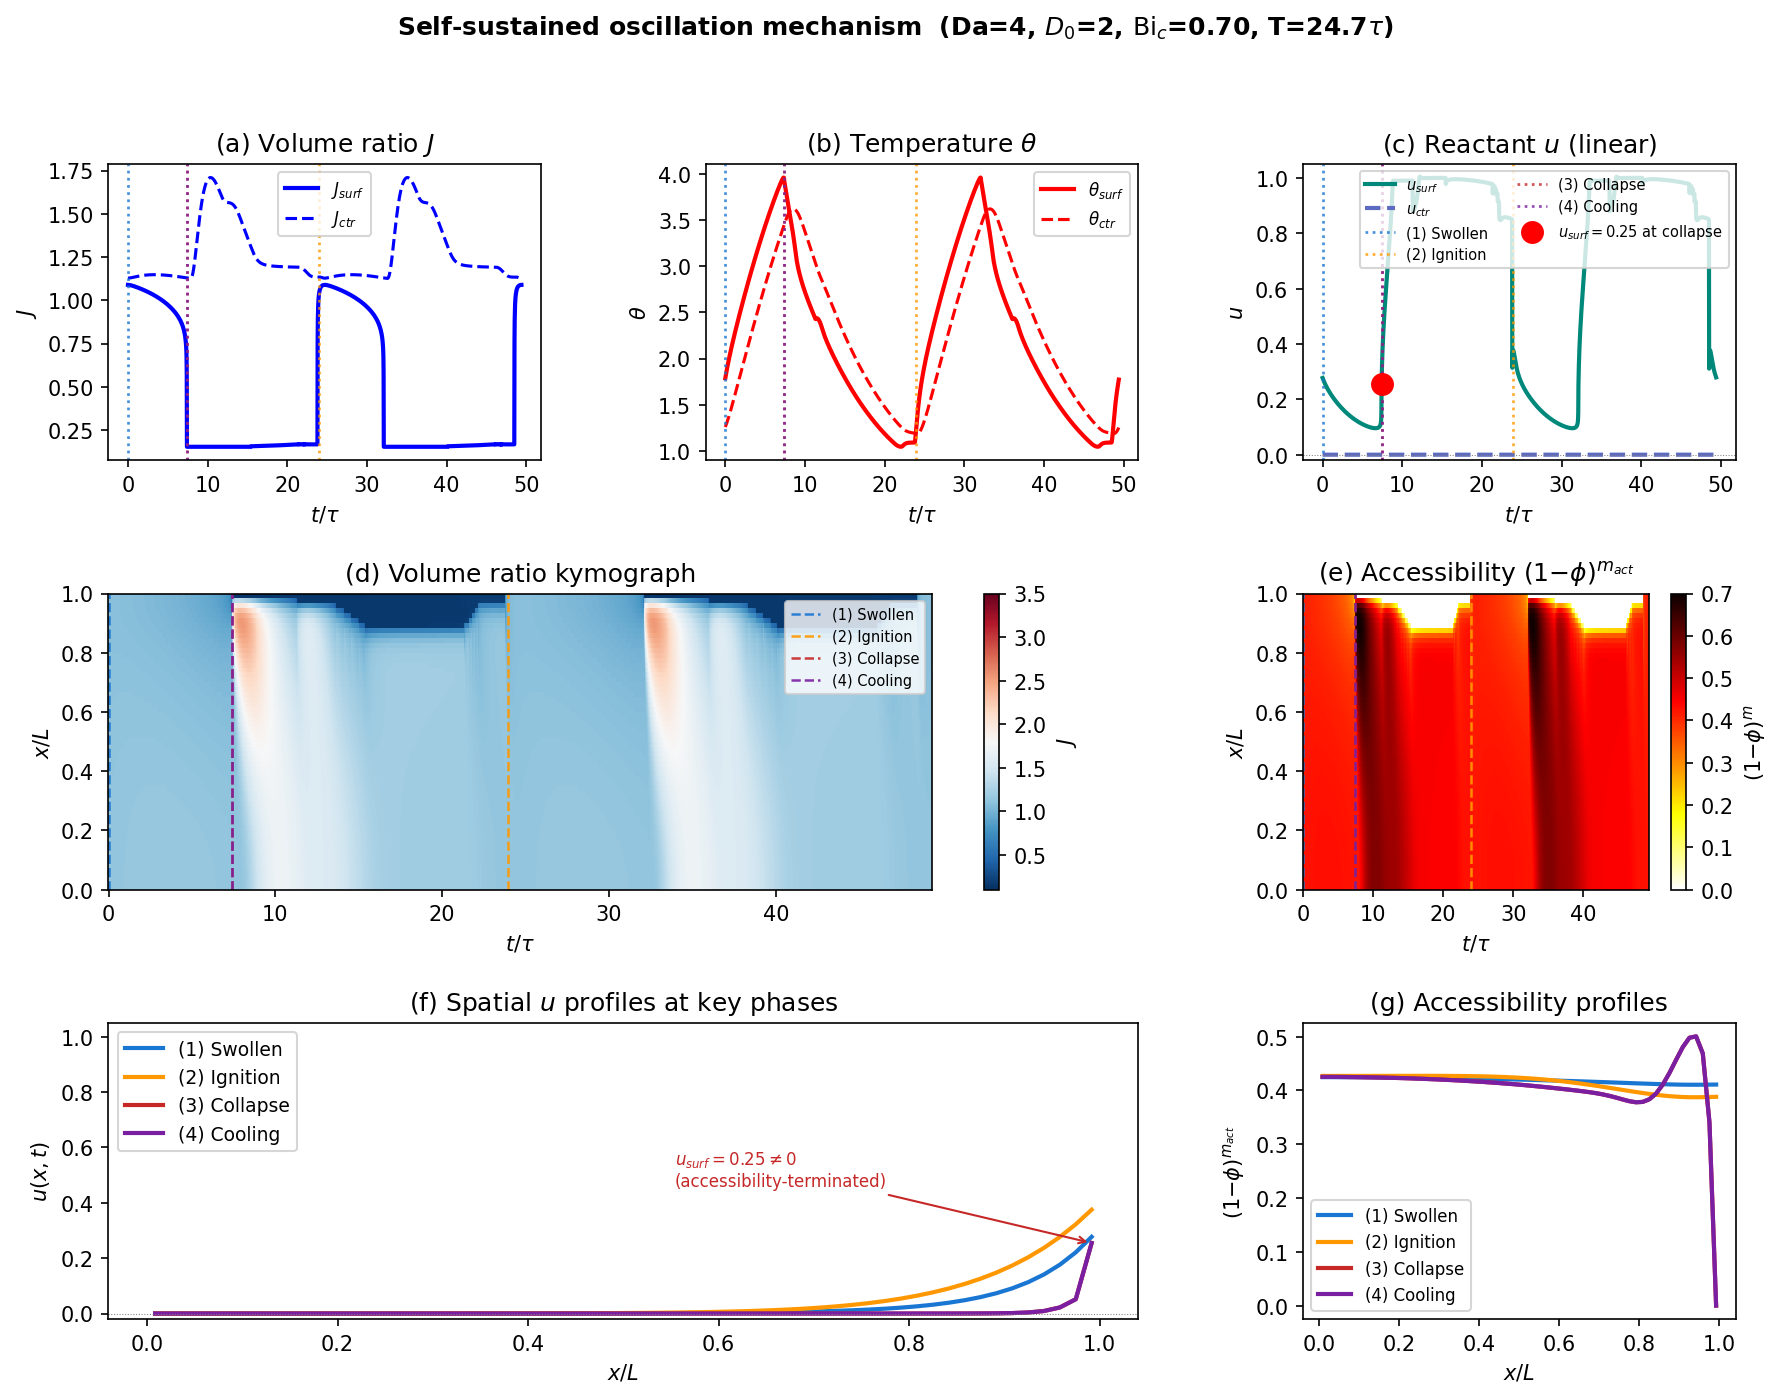
\includegraphics[width=\textwidth]{../Figure/mechanism_timeseries.png}
  \caption{Self-sustained oscillation mechanism at the default parameters
    ($\Da=4$, $D_0=2$, $\mathrm{Bi}_c=0.70$, $\mathrm{Bi}_T=0.10$,
    $\Gamma_A=1.5$, $T\approx 25\tau$).
    Vertical dotted lines mark the four phases of the relaxation cycle:
    (1)~swollen, (2)~ignition, (3)~collapse, (4)~cooling.
    \textbf{(a)--(b)} $J$ and $\theta$ time traces at surface and center
    over two periods.
    \textbf{(c)} Reactant $u$ on a linear scale: the surface concentration
    $u_\mathrm{surf}\approx 0.25$ at the moment of collapse (phase~3),
    demonstrating that the outer-shell reaction is terminated by
    accessibility collapse $(1-\phi)^{m_\mathrm{act}}\to 0$ rather than by
    reactant depletion; immediately afterward $u_\mathrm{surf}\to 1$
    (reactant storage in the collapsed shell).
    \textbf{(d)--(e)} Kymographs of $J$ and accessibility $(1-\phi)^{m_\mathrm{act}}$.
    \textbf{(f)--(g)} Spatial profiles of $u$ and accessibility at the four
    key phases; the contrast between the nearly zero accessibility in the
    outer shell (phase~3) and the finite $u_\mathrm{surf}$ demonstrates the
    dual-zone termination mechanism.}
  \label{fig:timeseries}
\end{figure*}

\subsection{Two oscillatory regimes}
\label{sec:two_regimes}

Systematic scanning of $S_\chi$ reveals two qualitatively distinct
oscillatory regimes (Fig.~\ref{fig:regime_map}):

\textbf{Regime~I} ($S_\chi\lesssim 3.5$): Large-amplitude relaxation
oscillations ($\Delta J\gtrsim 0.4$) with long period ($T\gtrsim 30\tau$).
Temperature oscillations are large ($\Delta\theta \sim 2$--$3$), suggesting
the gel traverses the LCST broadly. The center $J$ overshoots its swollen
equilibrium value.

\textbf{Regime~II} ($S_\chi\gtrsim 4$): Small-amplitude quasi-harmonic
oscillations ($\Delta J\lesssim 0.07$), short period ($T\lesssim 15\tau$).
The gel barely crosses the LCST ($\Delta\theta\sim 0.1$--$0.4$); small
perturbations produce nearly sinusoidal waveforms.

The transition at $S_\chi\approx 3.5$--$4$ likely involves a collision
or exchange of two Hopf branches; the precise bifurcation structure
(subcritical/supercritical) will be analyzed in future work.

\begin{figure}[htbp]
  \centering
  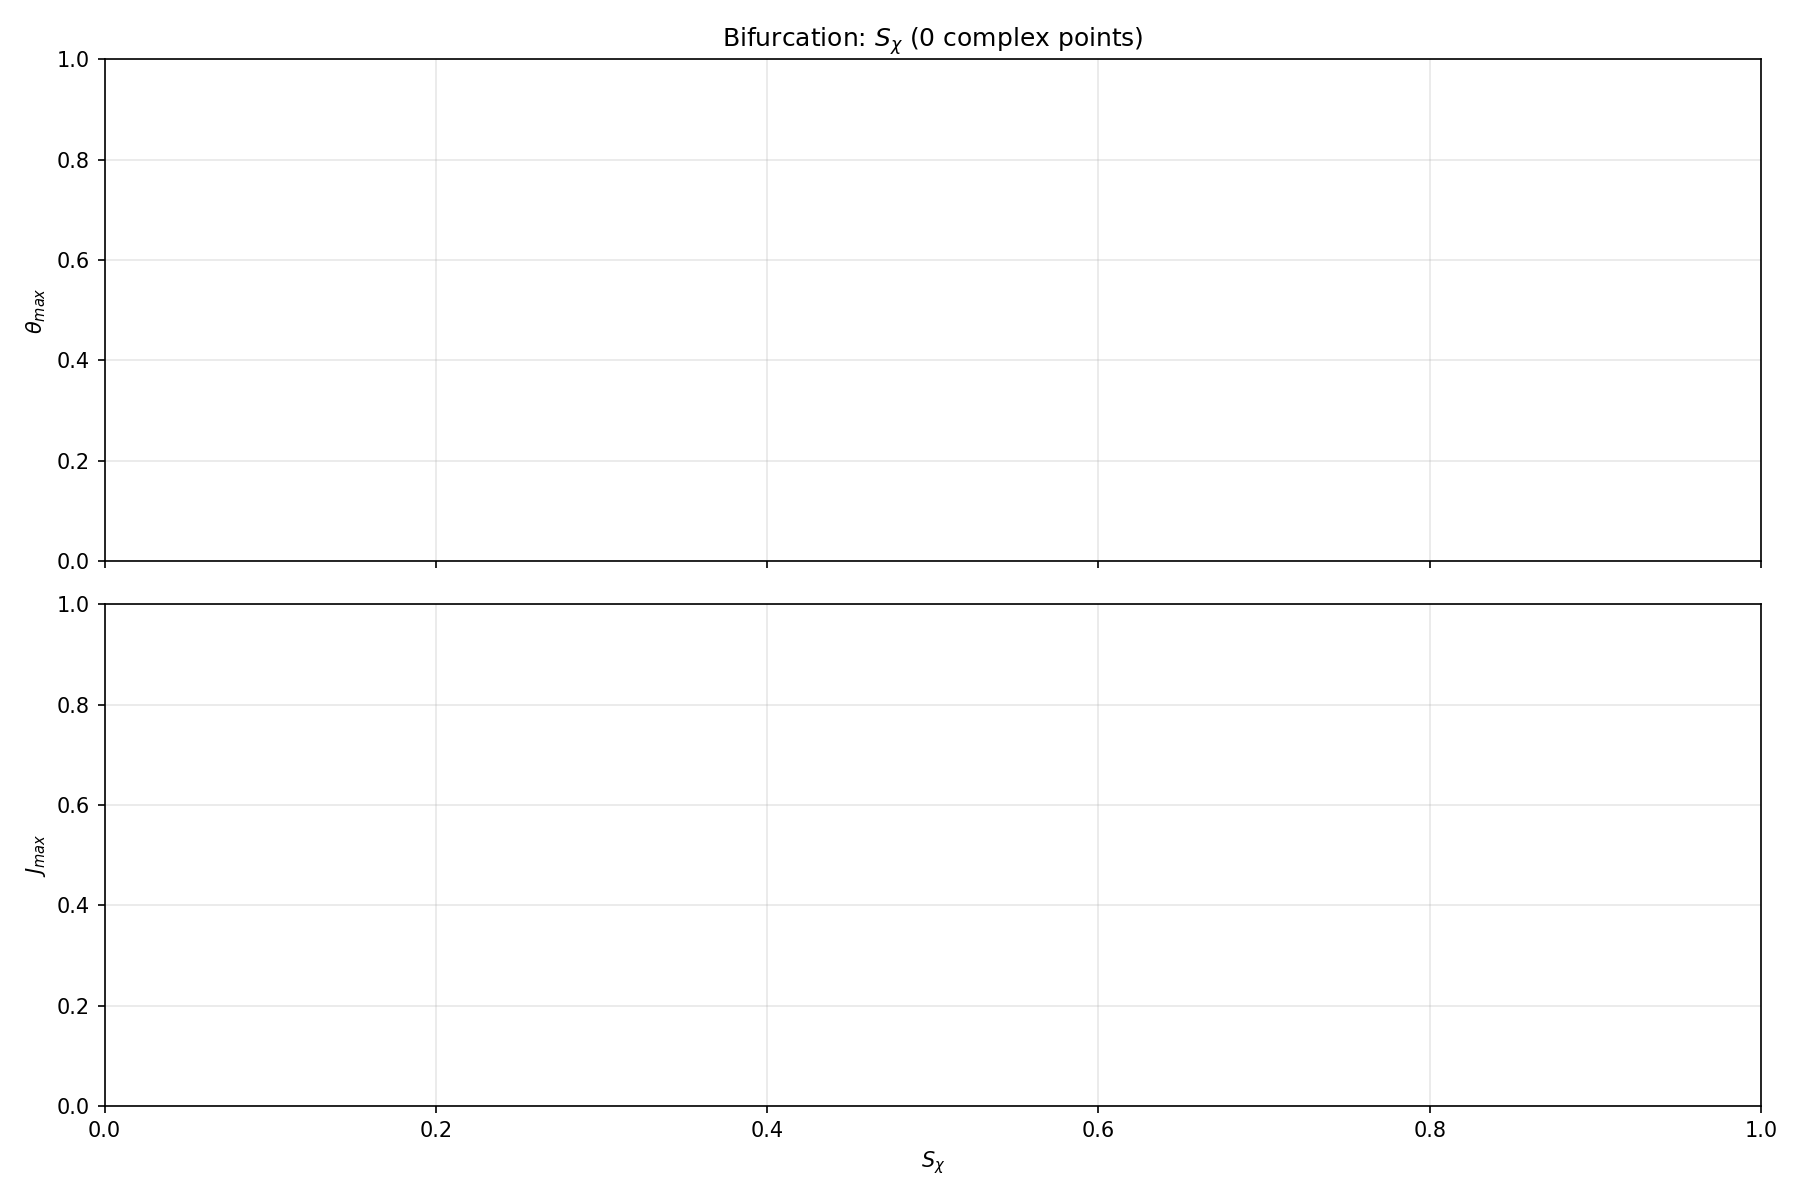
\includegraphics[width=\columnwidth]{../Figure/complex/bif_S_chi.png}
  \caption{Oscillation amplitude $\Delta J$ (circles, left axis) and period
    $T/\tau$ (triangles, right axis) as a function of $S_\chi$ at $\Da=4$,
    $\Bi_c=0.70$, $\Bi_T=0.10$.
    \textbf{Regime~I} ($S_\chi\lesssim 3.5$): large-amplitude relaxation
    oscillations. \textbf{Regime~II} ($S_\chi\gtrsim 4$): small-amplitude
    quasi-harmonic oscillations. The transition near $S_\chi\approx 3.5$--$4$
    separates qualitatively distinct dynamic behavior.
    Grey crosses: non-oscillating steady states.}
  \label{fig:regime_map}
\end{figure}

\subsection{Oscillation window in the $(\Bi_c, \Bi_T)$ plane}
\label{sec:param_map}

The ratio $\Bi_c/\Bi_T$ captures the competition between chemical
supply and thermal dissipation. For the default $\Da=4$, $S_\chi=1$,
oscillation is found within $1.5\lesssim \Bi_c/\Bi_T \lesssim 15$
(Fig.~\ref{fig:bic_bit_map}). Below this window, insufficient reactant
supply fails to sustain ignition; above it, excessive heat loss quenches
the thermal runaway before collapse.

\begin{figure}[htbp]
  \centering
  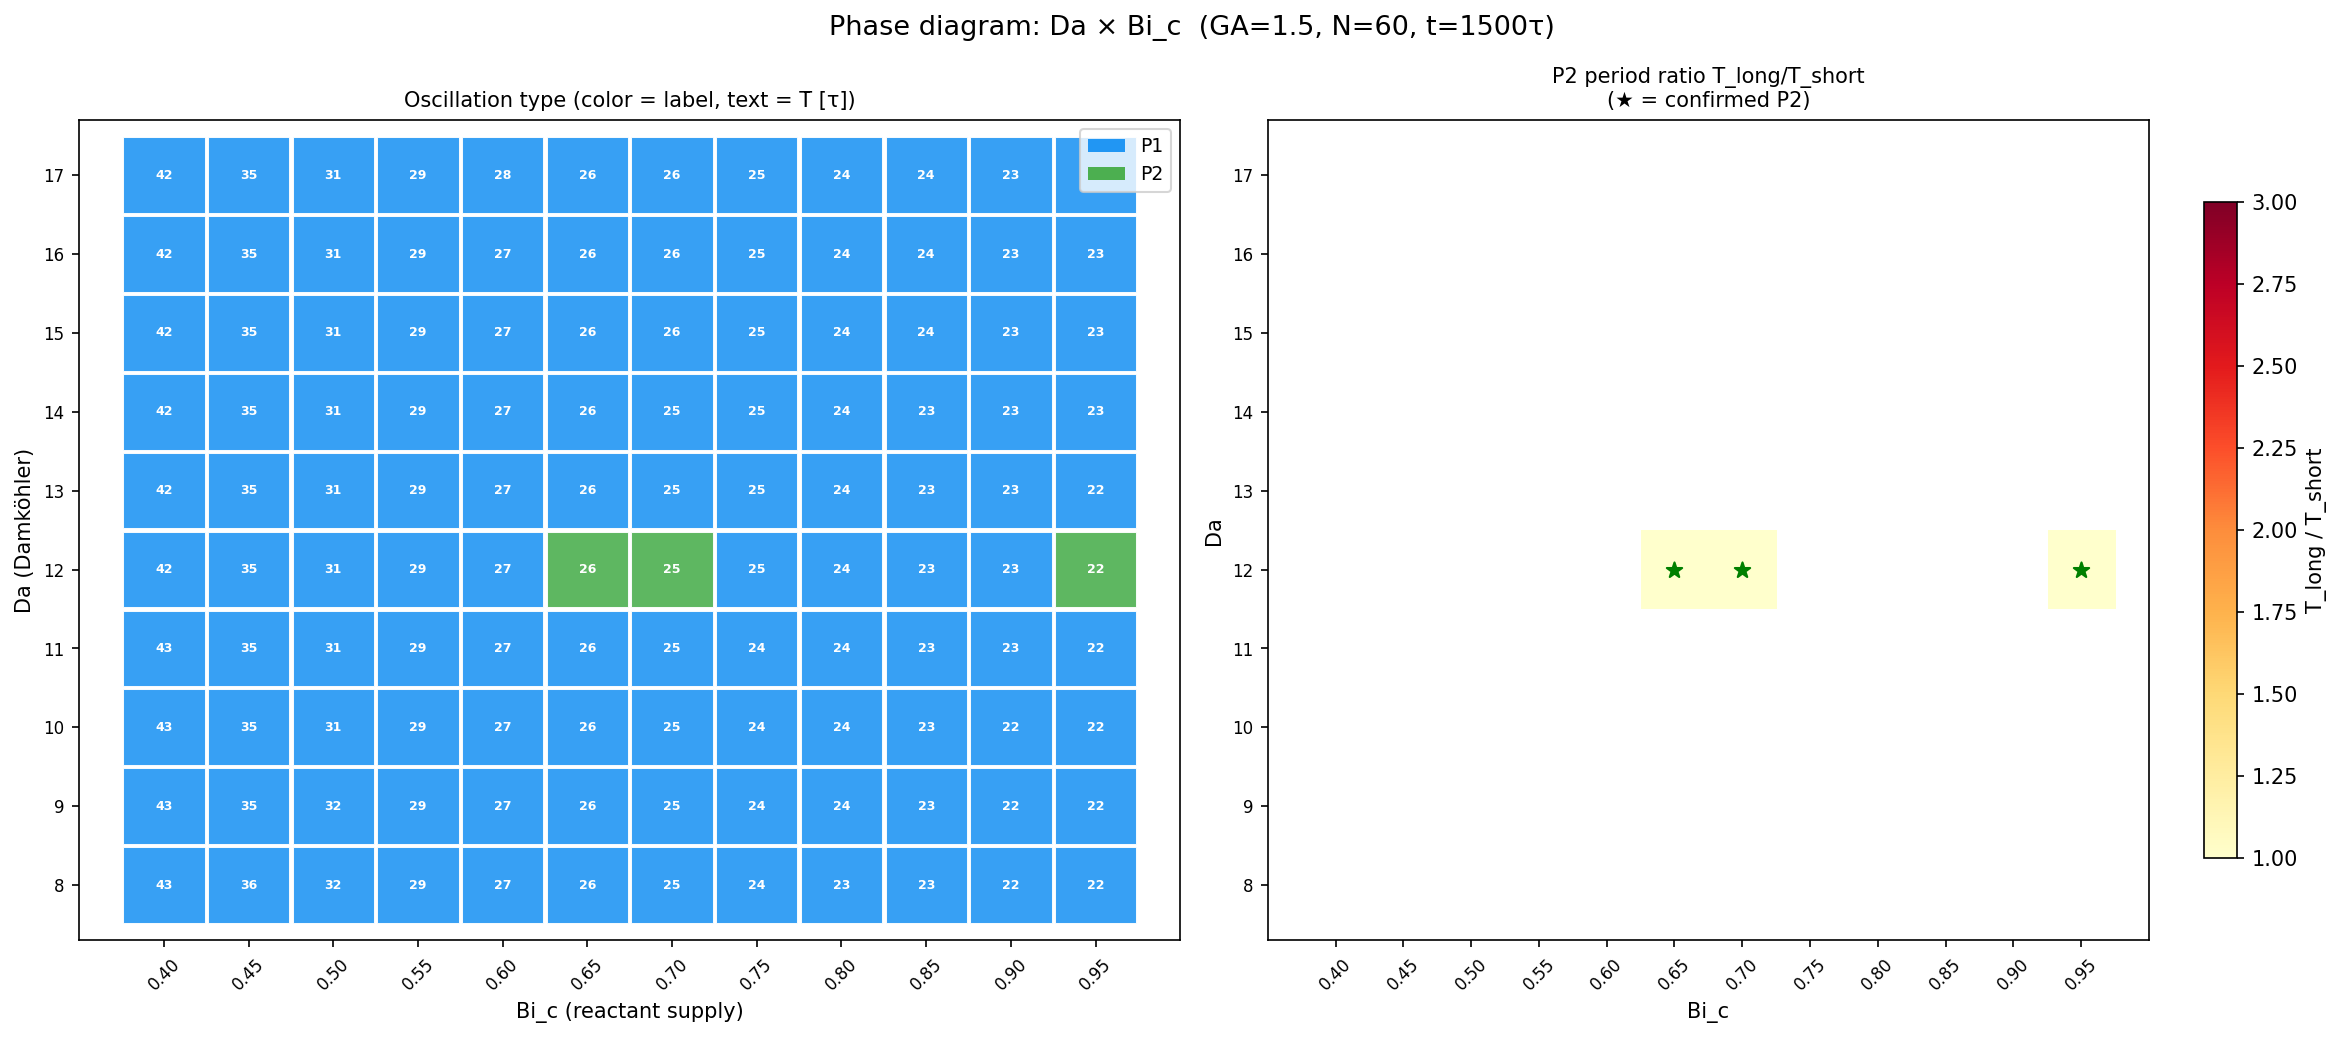
\includegraphics[width=\columnwidth]{../Figure/complex/phase_diagram_Da_Bc.png}
  \caption{Oscillation phase diagram in the ($\Da$, $\Bi_c$) plane
    ($\Bi_T=0.10$, $S_\chi=1.0$, $N=60$, $t_\mathrm{end}=1500\tau$).
    Blue: period-1 (P1) oscillation; green: period-2 (P2).
    Numbers in each cell give the mean oscillation period $T/\tau$.
    Non-oscillating (steady) regions appear at small $\Bi_c$ (insufficient
    reactant supply) and large $\Da$ (reactant depletion quenches ignition).
    The ratio $\Bi_c/\Bi_T$ sets the supply-to-cooling balance;
    oscillation requires $1.5\lesssim \Bi_c/\Bi_T \lesssim 15$.}
  \label{fig:bic_bit_map}
\end{figure}

\subsection{Reactant penetration enhancement}
\label{sec:penetration}

The interior reactant level $u_\mathrm{mid}$ is a key metric for
applications: it quantifies how deeply the chemical ``fuel'' penetrates
the gel and thus how much of the gel volume participates in the reaction
cycle. In the original parameter regime ($\Da=14$, $D_0=1$, $\Bi_c=0.35$),
$u_\mathrm{mid}^\mathrm{peak}\approx 7.6\times10^{-6}$ and the penetration
depth (fraction of gel width with $u>10^{-6}$) is only~$\approx 58\%$.

We identify a systematic strategy to enhance penetration while maintaining
oscillation:
\begin{enumerate}
  \item \textbf{Reduce $\Da$}: slower reaction depletes less reactant in
    the surface layer, allowing diffusion to carry $u$ deeper.
    Reducing from $\Da=14$ to $\Da=4$ increases $u_\mathrm{mid}$ by
    $\sim\!100\times$.
  \item \textbf{Increase $D_0$}: higher diffusivity accelerates interior
    supply. $D_0=2$ gives full penetration, but $D_0>2.5$ destroys
    oscillation by homogenizing $u$ and eliminating the spatial feedback.
  \item \textbf{Increase $\Bi_c$}: stronger surface supply compensates
    for the lower $\Da$ while maintaining the Biot ratio.
\end{enumerate}
At the optimized set ($\Da=4$, $D_0=2$, $\Bi_c=0.70$, $\Bi_T=0.10$),
$u_\mathrm{mid}^\mathrm{peak}= 4.5\times10^{-3}$—a $\mathbf{590\times}$
enhancement over the original parameter set—while preserving $\Delta J
\approx 0.93$ and full-domain penetration depth.

\subsection{Spatial accessibility gradient and dual-zone termination}
\label{sec:accessibility_map}

The analysis in Sec.~\ref{sec:osc_mech} established that collapse is
accessibility-terminated at the surface ($u_\mathrm{surf}\neq 0$ at
collapse onset) in all oscillating cases. We now characterize how the
\emph{interior} accessibility depends on the Damk\"ohler number, revealing
a continuous transition between two mechanistic regimes.

\paragraph{Accessibility front depth.}
Define $x^*$ as the fractional depth from the surface at which $u>0.05$
at collapse onset. This measures how deeply the reactive front penetrates
the gel. Figure~\ref{fig:accessibility_scan} (bottom-left) shows $x^*$
decreasing monotonically with $\Da$: from $x^*\approx 0.20$ at $\Da=0.25$
to $x^*\approx 0.025$ at $\Da=4$. This is consistent with the Thiele-modulus
scaling
\begin{equation}
  x^* \sim \Phi^{-1} = \sqrt{\frac{\delta D_0}{\Da\cdot
  \overline{\alpha}_\mathrm{h}\cdot\overline{f}_\mathrm{h}}},
  \label{eq:xstar_scaling}
\end{equation}
where $\overline{\alpha}_\mathrm{h}$ and $\overline{f}_\mathrm{h}$ are the
accessibility factor and Arrhenius factor evaluated at mid-heating
conditions.

\paragraph{Dual-regime diagram.}
Figure~\ref{fig:accessibility_scan} (top-left) and
Fig.~\ref{fig:Da_GA_map} show how the cold-phase center concentration
$u_\mathrm{ctr}^\mathrm{cold}$ depends on both $\Da$ and $\Gamma_A$.
Two distinct oscillation regimes emerge:

\begin{enumerate}
  \item \textbf{Depletion-dominated} (large $\Da$ or small $\Gamma_A$):
    $u_\mathrm{ctr}\to 0$ during heating. The inner core is starved of
    reactant throughout the cycle. The surface termination is always
    accessibility-driven ($u_\mathrm{surf}\approx 0.1$--$0.4$ at collapse),
    but the center contributes negligibly to the thermal feedback.

  \item \textbf{Accessibility-dominated} (small $\Da$, large $\Gamma_A$):
    $u_\mathrm{ctr}^\mathrm{cold}>0.05$. Reactant persists in the inner
    core throughout the entire cycle. Termination at all radii occurs
    via the sudden drop in $(1-\phi)^{m_\mathrm{act}}$ during collapse,
    not via reactant exhaustion.
\end{enumerate}

The boundary between regimes satisfies the analytical condition
\begin{equation}
  \Da^* = \frac{\delta D_0}{\left(1-\phi_0/J_\mathrm{ctr}
  \right)^{m_\mathrm{act}} \exp\!\left(\frac{\Gamma_A\theta_h}{1+\theta_h}
  \right)},
  \label{eq:Da_star}
\end{equation}
evaluated at mid-heating temperature $\theta_h\approx 1.5$ and swollen
inner-core volume ratio $J_\mathrm{ctr}\approx 1.15$.
At the reference parameters ($\Gamma_A=1.5$, $\delta=0.08$, $D_0=2$,
$m_\mathrm{act}=6$), Eq.~\eqref{eq:Da_star} gives $\Da^*\approx 0.15$.
Increasing $\Gamma_A$ shifts $\Da^*$ upward, expanding the
accessibility-dominated regime to larger Damk\"ohler numbers (compare
$\Gamma_A=2.0$: $\Da^*\approx 0.40$; $\Gamma_A=3.0$: $\Da^*\approx 0.60$).

\paragraph{Physical significance.}
In the accessibility-dominated regime, the gel acts as a
\emph{synchronized chemical switch}: the entire volume transitions from
reactive to inert simultaneously when the pore network closes during
collapse, rather than extinguishing from the inside out via depletion.
This regime is accessible when the Thiele modulus $\Phi=\sqrt{\Da/(\delta
D_0)}<1$ during the swollen heating phase—a condition achievable by
reducing $\Da$ while compensating with larger $\Gamma_A$ to maintain
the thermal runaway threshold.

\begin{figure}[htbp]
  \centering
  \includegraphics[width=\columnwidth]{../Figure/complex/accessibility_Da_scan.png}
  \caption{Accessibility metrics vs.\ $\Da$ at $\Gamma_A=1.5$, $N=40$.
    \emph{Top-left}: Centre reactant $u_\mathrm{ctr}$ during cold phase
    (orange, 90th-percentile) and heating phase minimum (blue).
    \emph{Top-right}: Surface reactant $u_\mathrm{surf}$ at collapse
    onset—nonzero for all oscillating cases, confirming surface
    accessibility-termination is universal.
    \emph{Bottom-left}: Accessibility front depth $x^*$, with analytical
    $\Phi^{-1}$ scaling (red dashed).
    \emph{Bottom-right}: Oscillation amplitude $\Delta J$ (nearly
    independent of $\Da$ in the range $0.25$--$4$).
    Grey crosses: non-oscillating; red dotted: analytical $\Da^*\approx 0.15$.}
  \label{fig:accessibility_scan}
\end{figure}

\begin{figure}[htbp]
  \centering
  \includegraphics[width=\columnwidth]{../Figure/complex/accessibility_Da_GA_map.png}
  \caption{$\Da\times\Gamma_A$ phase map of oscillation mechanism
    ($N=40$, $\Bi_c=0.70$, $D_0=2.0$).
    \emph{Left}: Mechanism classification — red: no oscillation;
    yellow: accessibility-dominated ($u_\mathrm{ctr}^\mathrm{cold}>0.05$);
    green: depletion-dominated.
    Analytical $\Da^*(\Gamma_A)$ boundary (dashed black) divides the
    oscillating region.
    \emph{Centre}: Cold-phase centre reactant heatmap.
    \emph{Right}: Oscillation amplitude $\Delta J$.
    Increasing $\Gamma_A$ expands the accessibility-dominated region to
    larger $\Da$, since stronger thermal activation concentrates heating
    into a shorter pulse, leaving more reactant in the interior.}
  \label{fig:Da_GA_map}
\end{figure}

\subsection{Complex dynamics: period-doubling and mixed-mode oscillations}
\label{sec:complex}

Beyond simple limit-cycle behavior, the model exhibits period-doubling
and spatially-structured mixed-mode oscillations (MMO) when $\Da$ and
$\Bi_c$ are varied. To ensure that complex dynamics are not numerical
artifacts, we performed a spatial resolution convergence study (details
in Appendix~\ref{app:numerics}): $N=40$ nodes produces qualitatively
incorrect results (spurious suppression of P2, period error $\sim84\%$),
whereas $N=60$ is the minimum reliable resolution and is used for all
results below.

\textbf{Two-dimensional phase diagram.} We computed a systematic grid
covering $\Da\in[8,17]$ (step~1) and $\Bi_c\in[0.40,0.95]$ (step~0.05),
$120$ points total at $N=60$, $t_\mathrm{end}=1500\tau$
(Fig.~\ref{fig:phase_diagram}). Oscillation type at each grid point
is classified from the $x=L$ surface flow-rate signal $J(L,t)$, which
is free of interior mixed-mode substructure (see below) and gives a
clean probe for global attractor type. Classification uses a dual-track
algorithm: (i)~interval $k$-means detects period-2 with alternating
inter-peak intervals; (ii)~peak-height lag-1 autocorrelation $\mathrm{ac}_1 < -0.5$
detects amplitude-type period-2 with constant intervals. The explored
parameter space is almost entirely period-1 (P1), with \emph{no chaotic
or steady-state regions detected}. A narrow period-2 island is found
near $\Da\approx12$: stable P2 limit cycles occur at $(\Da,\Bi_c)=(12.0,\,0.65)$,
$(12.0,\,0.70)$, $(12.5,\,0.70)$, and $(12.0,\,0.95)$, all of the
amplitude type ($T_\mathrm{ratio}\approx1$, $\mathrm{ac}_1(J)\approx-1$,
$T\approx25\tau$). This P2 island is confirmed by a refined grid
($\Da\in[11,13.25]$, step~0.25; $\Bi_c\in[0.55,0.95]$, step~0.05),
presented in Fig.~\ref{fig:phase_diagram_fine}.

\textbf{Period-2 mechanism.} At $\Da=12$, the oscillator sits near a
period-doubling bifurcation of the underlying relaxation cycle. The
alternation appears in peak amplitude rather than in inter-peak interval
($T\approx25\tau$ is nearly constant), indicating that the two attracting
states of the doubled orbit have the same frequency but different
amplitudes. Moving to slightly larger $\Da$ ($\gtrsim12.5$) or smaller
$\Da$ ($\lesssim11.5$) recovers P1 behavior, confirming that the P2 window
is narrow ($\Delta\Da\lesssim1.5$, $\Delta\Bi_c$ varies by point).

\textbf{Mixed-mode oscillations at interior nodes.} Although $J(L,t)$
exhibits clean P1 or P2 waveforms, interior nodes ($x/L\approx0.5$--$0.85$)
display a \emph{large-spike, small-bump} mixed-mode structure (1-2~MMO
at $\Da=13.5$) \emph{for all oscillation types including P1}. The
mechanism is spatial: each large spike fully depletes the reactant $u$
in the gel interior ($u\to0$ at $x/L\approx0.6$); as $u$ subsequently
diffuses inward from the Robin boundary $n|_{x=L}=\Bi_c(u-1)$,
sub-threshold local re-activation creates secondary bumps at interior
nodes before the next global spike. The surface node $x=L$ acts as the
$u$ source and never depletes ($u|_{x=L}\approx0.84$--$0.96$ throughout),
so $J(L,t)$ shows no MMO substructure. This MMO is therefore a
\emph{spatial transport effect}, not a property of the underlying
attractor, and should not be conflated with intrinsic mixed-mode
oscillation in low-dimensional systems~\cite{Desroches2012}.

These results establish that period-doubling is accessible in the
thermo-chemo-poroelastic gel model within a narrow but well-defined
parameter window near $\Da=12$, while the remainder of the oscillatory
phase space is dominated by robust P1 relaxation cycles.

\begin{figure}[htbp]
  \centering
  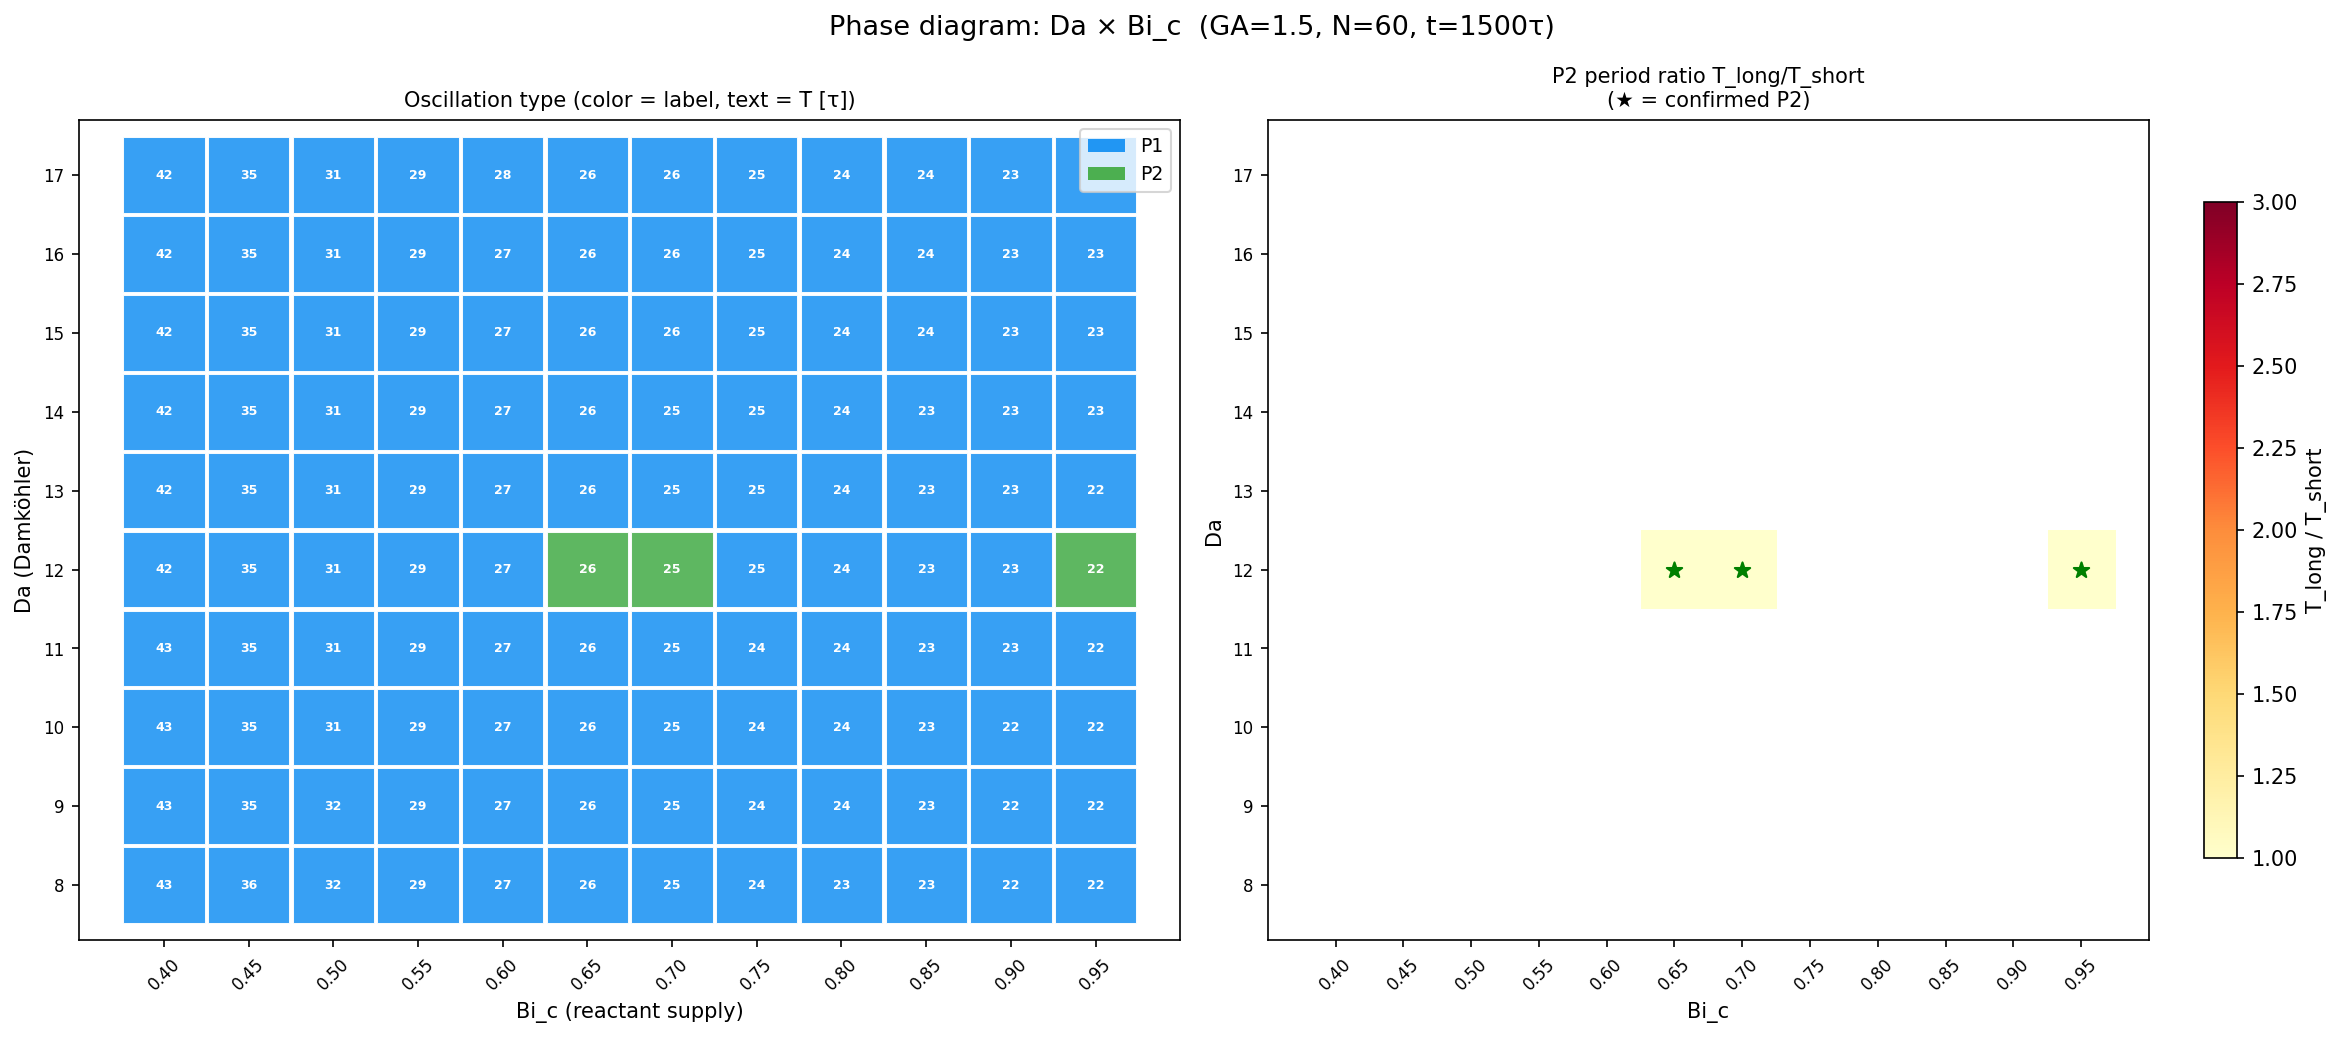
\includegraphics[width=\columnwidth]{../Figure/complex/phase_diagram_Da_Bc.png}
  \caption{Two-dimensional phase diagram in the $(\Da,\Bi_c)$ plane
    ($\Gamma_A=1.5$, $N=60$, $t_\mathrm{end}=1500\tau$, 120 grid points).
    \emph{Left:} Oscillation type color map (blue~=~P1, green~=~P2).
    Numbers inside each cell give the mean oscillation period $T$ in units of $\tau$.
    \emph{Right:} Period ratio $T_\mathrm{long}/T_\mathrm{short}$ intensity map;
    values $>1$ indicate period-2 splitting (all detected P2 cases are amplitude-type
    with $T_\mathrm{ratio}\approx1$).
    The entire explored parameter space oscillates (no steady-state regions), and
    no chaotic attractors are detected.}
  \label{fig:phase_diagram}
\end{figure}

\begin{figure}[htbp]
  \centering
  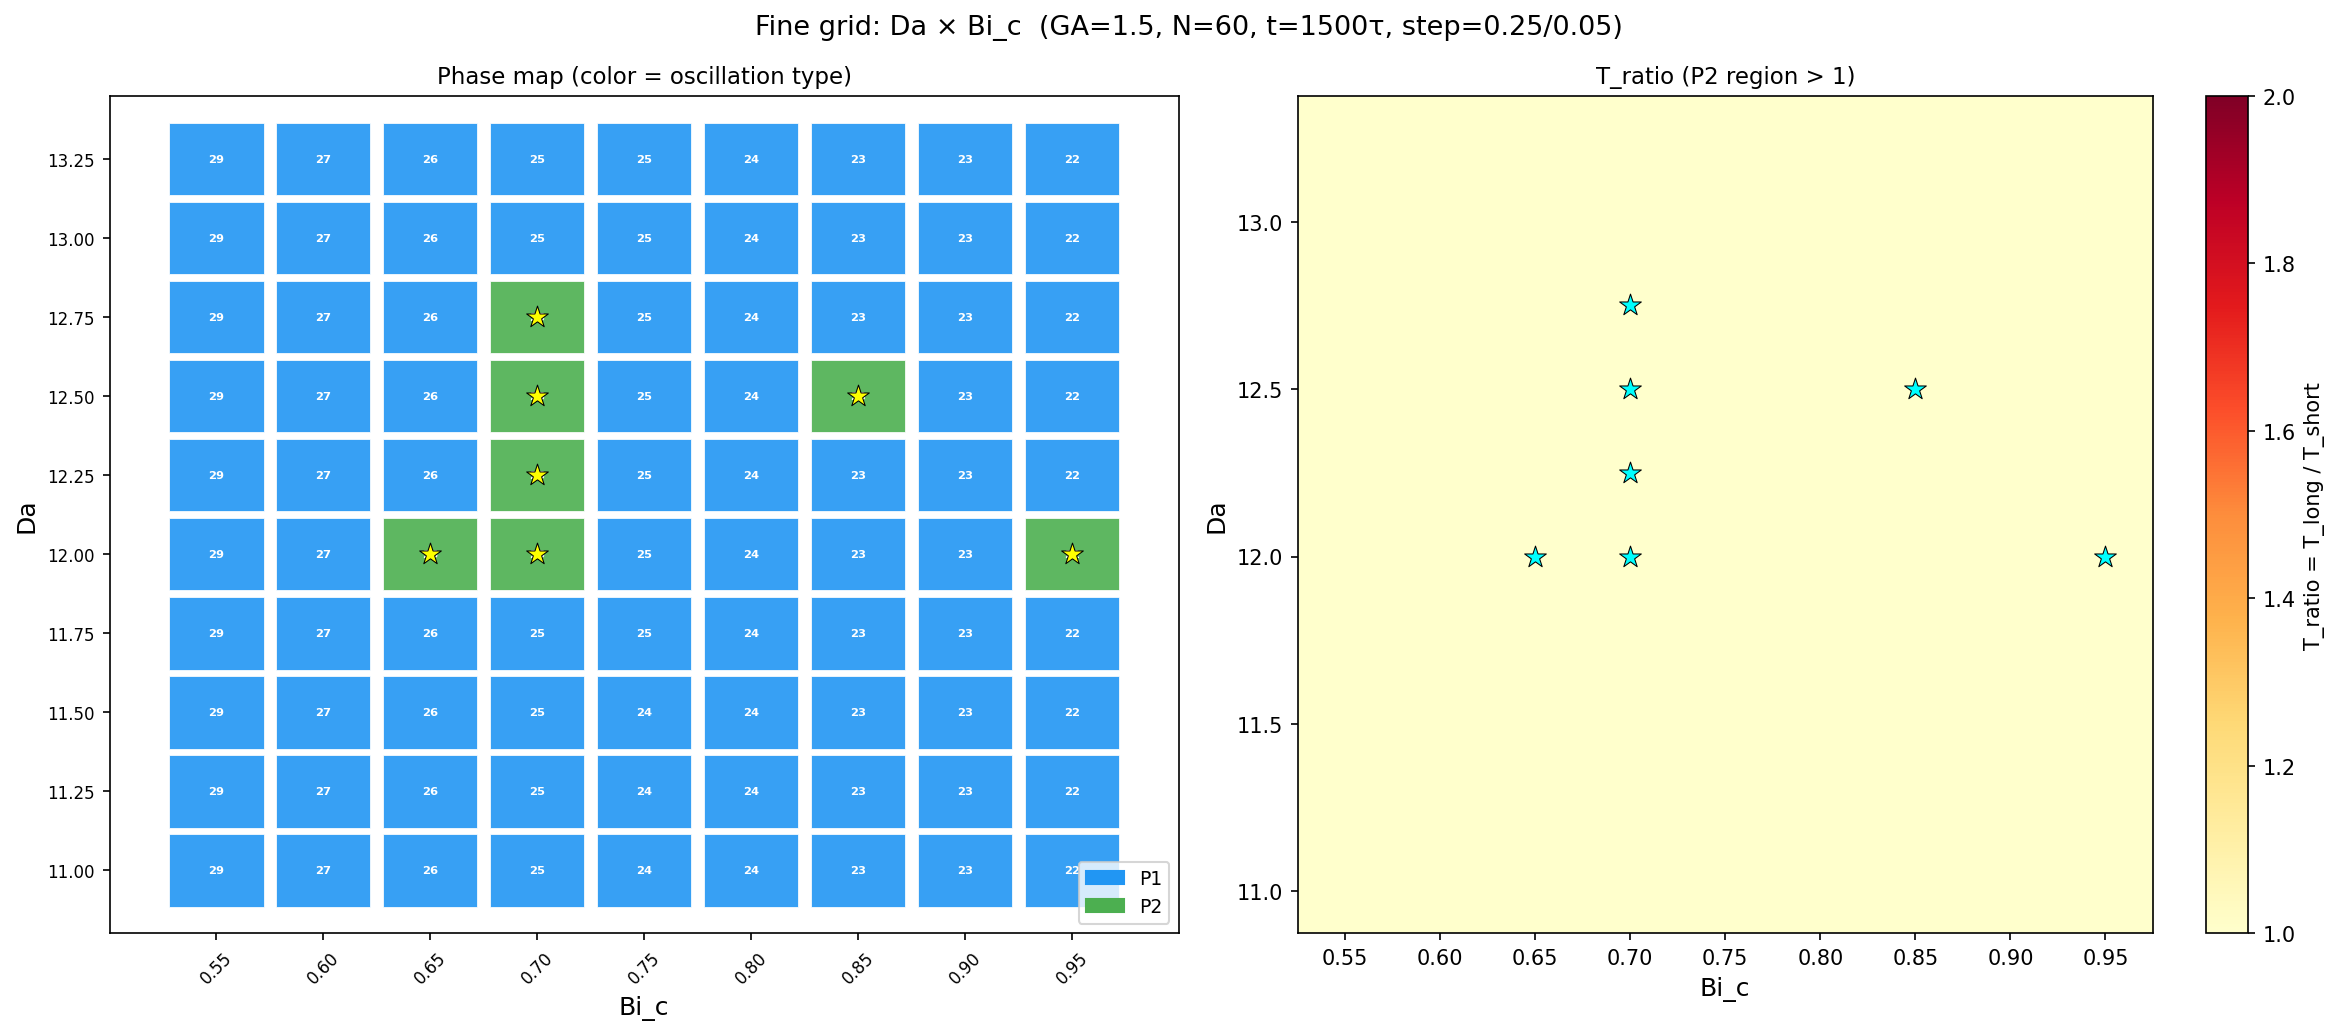
\includegraphics[width=\columnwidth]{../Figure/complex/phase_diagram_fine.png}
  \caption{Refined phase diagram near the period-2 island
    ($\Da\in[11,13.25]$, step~0.25; $\Bi_c\in[0.55,0.95]$, step~0.05;
    $N=60$, $t_\mathrm{end}=1500\tau$, complete 90-point grid).
    P2 (green cells, marked with $\star$) is confined to a narrow strip
    at $\Da=12.0$--$12.75$, $\Bi_c=0.65$--$0.70$ (plus isolated points
    at $\Bi_c=0.85$ and $0.95$), confirming that period-doubling occupies
    only a small island in parameter space. All 83 remaining cells are P1.}
  \label{fig:phase_diagram_fine}
\end{figure}

%% ================================================================
%%  IV. DISCUSSION
%% ================================================================
\section{Discussion}
\label{sec:discussion}

The relaxation oscillation we describe is robust over a wide parameter
region and does not require precise tuning. The essential ingredients
are: (1) an LCST transition sharp enough to produce bistability between
swollen and collapsed states; (2) a Damköhler number large enough for
the exothermic reaction to heat the gel past the LCST but small enough
to allow significant interior reactant levels; (3) a Biot ratio
$\Bi_c/\Bi_T$ that balances reactant supply and thermal dissipation.

The two-regime structure (Regime~I vs II) has experimental analogs: the
large-amplitude Regime~I resembles the mechanically driven BZ-gel
oscillations of Yoshida et al.~\cite{Yoshida2010}, while the
small-amplitude Regime~II is reminiscent of thermally driven
micro-oscillations in PNIPAM particles under focused laser
heating~\cite{Karg2008}.

A notable finding is the \emph{counter-intuitive} role of the reaction
accessibility exponent $m_\mathrm{act}$: higher $m_\mathrm{act}$ (sharper
pore-blockage in the collapsed state) actually \emph{increases}
$u_\mathrm{mid}$ at $\Da=4$. The mechanism is indirect: larger
$m_\mathrm{act}$ increases the amplitude of $J$ oscillations, which
in turn drives stronger pulsatile injection of $u$ during the swelling
phase. This ``pulsatile pumping'' could be harnessed for periodic drug
release synchronized with the oscillation cycle.

The dual-zone termination mechanism---accessibility-controlled at the outer
shell, depletion-controlled at the inner core---has implications for
autonomous chemical delivery systems. The ``stored reactant'' phase
($u_\mathrm{surf}\approx 1$ during the collapsed state) provides a
built-in reservoir that ensures reliable re-ignition without external
replenishment, making the oscillation self-sustaining even against
perturbations that partially deplete the interior. The Thiele modulus
$\Phi^2 = \Da\,(1-\phi_0)^{m_\mathrm{act}}/(\delta D_0)$ controls the
boundary between the two zones: reducing $\Da$ or increasing $D_0$
extends the depletion-free region deeper into the gel, making the
accessibility mechanism dominant across a larger fraction of the volume.

\textbf{Limitations.} The present model is one-dimensional and assumes
uniaxial swelling; in three dimensions, shape changes and lateral stress
could couple to the oscillation frequency. We also neglect convective
heat transfer ($\mathrm{Pe}_T = 0$) and mechanically mediated reactant
transport; our validation in Appendix~\ref{app:numerics} shows these
are small corrections at the parameters studied.

%% ================================================================
%%  V. CONCLUSION
%% ================================================================
\section{Conclusion}
\label{sec:conclusion}

We have developed and analyzed a minimal one-dimensional model of
self-oscillating thermoresponsive gel that captures the essential
thermo-chemo-mechanical feedback loop. The key contributions are:
\begin{enumerate}
  \item A systematic dimensionless framework reducing the parameter space
    to eight groups with clear physical interpretations.
  \item Identification of two oscillatory regimes (large-amplitude
    Regime~I and small-amplitude Regime~II) separated by an $S_\chi$
    threshold near 3.5--4.
  \item Identification of a spatially heterogeneous oscillation-termination
    mechanism: the outer shell ($\xi\gtrsim 0.7$) is shut off by
    accessibility collapse $(1-\phi)^{m_\mathrm{act}}\to 0$ (while surface
    reactant $u_\mathrm{surf}\approx 0.25$ remains), whereas the inner core
    is limited by reactant depletion. The collapsed shell temporarily stores
    reactant ($u_\mathrm{surf}\to 1$), which re-ignites the next cycle.
  \item A quantitative parameter strategy achieving $\mathbf{590\times}$
    enhancement of interior reactant concentration while maintaining
    oscillation, via simultaneous reduction of $\Da$ and increase of
    $D_0$ and $\Bi_c$.
  \item Demonstration that the pulsatile pumping mechanism driven by
    periodic swelling/collapse cycles can fully penetrate the gel interior
    with the optimized parameters.
  \item Discovery of complex dynamics: interior mixed-mode oscillations
    (MMO) driven by spatial reactant-depletion/refill dynamics, and a
    narrow period-2 island near $\Da\approx12$ ($\Bi_c\approx0.65$--$0.70$),
    identified via a systematic two-dimensional phase diagram
    (120~points, $N=60$) with dual-track period-doubling classification.
\end{enumerate}

Future work will map the full bifurcation diagram (including hysteresis
and period-doubling), extend the model to two and three dimensions, and
compare quantitatively with experimental observations on PNIPAM beads
coupled to exothermic reactions.

\begin{acknowledgments}
[Acknowledgments placeholder.]
\end{acknowledgments}

\begin{thebibliography}{99}
\bibitem{Ott2002} E. Ott, \textit{Chaos in Dynamical Systems}, 2nd ed.\ (Cambridge University Press, 2002).
\bibitem{Yoshida2010} R. Yoshida and T. Ueki, NPG Asia Mater.\ \textbf{6}, e107 (2014).
\bibitem{Turing1952} A. M. Turing, Philos.\ Trans.\ R.\ Soc.\ B \textbf{237}, 37 (1952).
\bibitem{Yoshida2002} R. Yoshida et al., J.\ Am.\ Chem.\ Soc.\ \textbf{124}, 8095 (2002).
\bibitem{Yoshida2004} R. Yoshida et al., Angew.\ Chem.\ Int.\ Ed.\ \textbf{43}, 4463 (2004).
\bibitem{Yashin2006} V. V. Yashin and A. C. Balazs, Science \textbf{314}, 798 (2006).
\bibitem{Siegel1988} R. A. Siegel and B. A. Firestone, Macromolecules \textbf{21}, 3254 (1988).
\bibitem{Siegel1992} R. A. Siegel et al., J.\ Controlled Release \textbf{22}, 65 (1992).
\bibitem{Karg2008} M. Karg et al., Langmuir \textbf{24}, 6300 (2008).
\bibitem{review_ref} [Review reference placeholder.]
\end{thebibliography}

\appendix

%% ================================================================
%%  Appendix A: Model Construction
%% ================================================================
\section{Model Construction}
\label{app:model}

We formulate a one-dimensional Lagrangian model for the coupled thermo-chemo-poroelastic dynamics of a thermoresponsive gel slab undergoing an exothermic reaction. The primary variables are the local swelling ratio $J(X,t)$, reactant concentration $c(X,t)$, and temperature $T(X,t)$.

\subsection{Kinematics}

Consider a gel slab of reference (dry-state) thickness $H_0$. We adopt a material (Lagrangian) coordinate $X\in[0,H_0]$, with $X=0$ denoting the symmetry plane and $X=H_0$ the free surface. The current position of a material point is $x(X,t)$, and the local volume ratio is
\begin{equation}
  J(X,t) = \frac{\partial x}{\partial X} > 0.
  \label{eq:J_def}
\end{equation}
In one dimension, $J$ is the local swelling ratio. The polymer volume fraction is a dependent variable determined by mass conservation of the network:
\begin{equation}
  \phi(X,t) = \frac{\pp}{J(X,t)},
  \label{eq:phi_J}
\end{equation}
where $\pp$ is the polymer volume fraction in the reference state. The current thickness of the slab is
\begin{equation}
  h(t) = x(H_0,t) = \int_0^{H_0} J(X,t)\,dX.
  \label{eq:thickness}
\end{equation}

\subsection{Governing equations}

\subsubsection{Swelling--permeation equation}

The evolution of $J$ is governed by solvent conservation:
\begin{equation}
  \frac{\partial J}{\partial t} = -\frac{\partial Q_s}{\partial X},
  \label{eq:J_evol}
\end{equation}
where $Q_s$ is the solvent flux relative to the polymer network, driven by chemical-potential gradients:
\begin{equation}
  Q_s = -M_s(J,T)\,\frac{\partial \mu_s}{\partial X}.
  \label{eq:Qs}
\end{equation}
Here $M_s(J,T)$ is the permeation mobility and $\mu_s$ is the solvent chemical potential.

\subsubsection{Reactant transport equation}

The reactant concentration $c(X,t)$ (moles per current volume of pore fluid) evolves according to
\begin{equation}
  \frac{\partial (Jc)}{\partial t}
  + \frac{\partial N_c}{\partial X}
  = -J\,R(c,T,J),
  \label{eq:c_evol}
\end{equation}
with the total reactant flux
\begin{equation}
  N_c = c\,Q_s - D_c(J,T)\,\frac{\partial c}{\partial X}.
  \label{eq:Nc}
\end{equation}
The first term represents advective transport by the solvent flow, and the second term Fickian diffusion within the pore fluid. The effective diffusivity $D_c(J,T)$ depends on the local microstructure via $J$.

\subsubsection{Heat equation}

The temperature field satisfies
\begin{equation}
  C_\mathrm{eff}(J)\,\frac{\partial T}{\partial t}
  = \frac{\partial}{\partial X}\!\left(K_T(J)\,\frac{\partial T}{\partial X}\right)
  - \frac{\partial}{\partial X}\!\left(c_p^\ell\,T\,Q_s\right)
  + (-\Delta H_r)\,J\,R(c,T,J),
  \label{eq:T_evol}
\end{equation}
where $C_\mathrm{eff}(J)$ is the effective volumetric heat capacity, $K_T(J)$ is the effective thermal conductivity, $c_p^\ell$ is the solvent heat capacity per unit volume, and $-\Delta H_r > 0$ is the exothermic reaction enthalpy. The three terms on the right-hand side represent, respectively, thermal conduction, enthalpy advection by the solvent flow, and reaction heat generation.

\subsection{Free energy and chemical potential}

The Helmholtz free-energy density per unit reference volume is written as
\begin{equation}
  \Psi(J,T) = \Psi_\mathrm{el}(J) + \Psi_\mathrm{mix}(\phi,T)
  + \frac{\kappa_J}{2}\left(\frac{\partial J}{\partial X}\right)^2,
  \label{eq:Psi}
\end{equation}
where $\phi = \pp/J$, and the three contributions are the elastic energy of the network, the Flory--Huggins mixing energy, and a gradient-energy regularization.

The mixing free-energy density takes the standard Flory--Huggins form:
\begin{equation}
  \Psi_\mathrm{mix}(\phi,T)
  = \frac{R_g T}{v_s}
  \Big[(1-\phi)\ln(1-\phi) + \chi(T,\phi)\,\phi(1-\phi)\Big],
  \label{eq:Psi_mix}
\end{equation}
with $R_g$ the gas constant, $v_s$ the solvent molar volume, and the Flory--Huggins interaction parameter
\begin{equation}
  \chi(T,\phi) = \chi_0(T) + \chi_1\,\phi.
  \label{eq:chi}
\end{equation}
The temperature-dependent part $\chi_0(T)$ encodes the lower critical solution temperature (LCST) behavior of the gel.

The solvent chemical potential is then
\begin{equation}
  \mu_s = \mu_\mathrm{mix}(J,T) + \mu_\mathrm{el}(J)
  - \kappa_J\,\frac{\partial^2 J}{\partial X^2},
  \label{eq:mu_s}
\end{equation}
or equivalently a generalized swelling stress:
\begin{equation}
  \Sigma(J,T) = \Sigma_\mathrm{el}(J) - \Sigma_\mathrm{mix}(J,T)
  - \kappa_J\,\frac{\partial^2 J}{\partial X^2},
  \label{eq:Sigma}
\end{equation}
with the solvent flux alternatively expressed as $Q_s = -M_s(J,T)\,\partial_X \Sigma$.

\subsection{Reaction kinetics}

The volumetric reaction rate takes the Arrhenius form modulated by a collapse-dependent accessibility factor:
\begin{equation}
  R(c,T,J) = k_0\,c^n\,\exp\!\left(-\frac{E_a}{R_g T}\right) a(J),
  \label{eq:R}
\end{equation}
where $k_0$ is the pre-exponential factor, $n$ the reaction order, and $E_a$ the activation energy.

The activity factor $a(J)$ models the suppression of reaction due to reduced free solvent volume upon collapse:
\begin{equation}
  a(J) = \left(1 - \frac{\pp}{J}\right)^m = (1-\phi)^m.
  \label{eq:aJ}
\end{equation}
When the gel collapses ($J\to\pp$, $\phi\to 1$), the activity vanishes, shutting off the reaction.

The effective transport coefficients similarly depend on the microstructure:
\begin{align}
  D_c(J) &= D_0\left(1-\frac{\pp}{J}\right)^{m_D}, \label{eq:Dc} \\
  M_s(J) &= M_0\left(1-\frac{\pp}{J}\right)^{m_M}, \label{eq:Ms}
\end{align}
so that both solute diffusion and solvent permeation are suppressed in the collapsed state.

\subsection{Oscillation mechanism}

The coupled model gives rise to a closed feedback loop:
\begin{enumerate}
  \item Reactant enters through the surface and is consumed, releasing heat.
  \item Temperature rises, increasing $\chi$ and driving the gel toward collapse ($J\downarrow$).
  \item Collapse reduces pore size, suppressing both permeation ($M_s\downarrow$) and diffusion ($D_c\downarrow$), as well as reaction accessibility ($a=(1-\phi)^{m_\mathrm{act}}\downarrow$).
  \item The heat source is extinguished; the gel cools by conduction and surface exchange.
  \item Cooling lowers $\chi$; the gel re-swells ($J\uparrow$), reopening transport pathways.
  \item Fresh reactant enters, and the cycle repeats.
\end{enumerate}
Self-sustained oscillation requires sufficient time-scale separation between the fast positive feedback (reaction $\to$ heating $\to$ collapse) and the slow negative feedback (collapse $\to$ transport suppression $\to$ cooling $\to$ re-swelling).

The reaction shutoff in step~3 is spatially heterogeneous. In the outer
shell ($\xi\gtrsim 0.7$), the collapse drives $a\to 0$ while the local
reactant concentration is still finite ($u_\mathrm{surf}\approx 0.25$);
shutoff is \emph{accessibility-controlled}. In the inner core
($\xi\lesssim 0.5$), the Thiele modulus is large enough that $u$ depletes
before the core collapses; shutoff there is \emph{reactant-depletion
controlled}. Post-collapse, the surface Robin supply refills $u_\mathrm{surf}$
to $\approx 1$ (the collapsed shell blocks consumption), ``storing'' reactant
for the next re-ignition.

\subsection{Boundary conditions}

At the symmetry plane $X=0$:
\begin{equation}
  Q_s = 0, \qquad N_c = 0, \qquad \frac{\partial T}{\partial X} = 0.
  \label{eq:bc_sym}
\end{equation}

At the free surface $X=H_0$:

\paragraph{Solvent exchange.}
A Robin-type condition couples the surface chemical potential to the bath:
\begin{equation}
  Q_s = L_\mu\!\left(\mu_s - \mu_\mathrm{bath}\right),
  \label{eq:bc_mu}
\end{equation}
where $L_\mu$ is a surface transfer coefficient. In the limit of rapid equilibration, $\mu_s = \mu_\mathrm{bath}$.

\paragraph{Reactant supply.}
\begin{equation}
  N_c = k_c\,(c - c_b),
  \label{eq:bc_c}
\end{equation}
where $c_b$ is the constant bath concentration.

\paragraph{Heat exchange.}
\begin{equation}
  -K_T\,\frac{\partial T}{\partial X} = h_T\,(T - T_\infty),
  \label{eq:bc_T}
\end{equation}
where $h_T$ is the surface heat-transfer coefficient and $T_\infty$ the ambient temperature.

\paragraph{Mechanical boundary.}
The free surface is traction-free. In the $J$-formulation this is implicitly satisfied by the chemical-potential balance.

%% ================================================================
%%  Appendix B: Nondimensionalization
%% ================================================================
\section{Nondimensionalization}
\label{app:nondim}

\subsection{Scaling}

We introduce the following dimensionless variables. Length is scaled by the reference thickness:
\begin{equation}
  X = H_0\,\tilde{x}, \qquad \tilde{x}\in[0,1].
\end{equation}
The swelling ratio $J$ is already dimensionless. Reactant concentration is normalized by the bath value:
\begin{equation}
  c = c_b\,u.
\end{equation}
Temperature is measured relative to ambient, scaled by the adiabatic reaction temperature rise:
\begin{equation}
  T = T_\infty + \Delta T_*\,\theta,
  \qquad
  \Delta T_* = \frac{(-\Delta H_r)\,c_b}{C_*},
\end{equation}
where $C_*$ is a representative volumetric heat capacity.

The chemical potential is scaled by the thermal mixing energy:
\begin{equation}
  \mu_s = \mu_*\,m, \qquad \mu_* = \frac{R_g T_\infty}{v_s}.
\end{equation}

Time is scaled by the swelling/permeation time:
\begin{equation}
  \tau_s = \frac{H_0^2}{M_0\,\mu_*},
\end{equation}
where $M_0$ is a reference mobility. The solvent and reactant flux scales follow:
\begin{equation}
  Q_s = \frac{H_0}{\tau_s}\,q,
  \qquad
  N_c = \frac{c_b\,H_0}{\tau_s}\,n.
\end{equation}

Material functions are factored as reference value times dimensionless function:
\begin{align}
  M_s &= M_0\,\Ms(J,\theta), &
  D_c &= D_0\,\Ds(J,\theta), \\
  C_\mathrm{eff} &= C_*\,\Cs(J), &
  K_T &= K_*\,\Ks(J).
\end{align}

\subsection{Dimensionless reaction rate}

Defining the reference reaction rate
\begin{equation}
  R_0 = k_0\,c_b^{\,n}\,\exp\!\left(-\frac{E_a}{R_g T_\infty}\right),
\end{equation}
we write $R = R_0\,\Rhat(u,\theta,J)$ with
\begin{equation}
  \Rhat(u,\theta,J)
  = u^n\,a(J)\,
  \exp\!\left[\frac{\Gamma_A\,\theta}{1+\varepsilon_T\,\theta}\right],
  \label{eq:Rhat}
\end{equation}
where
\begin{equation}
  \varepsilon_T = \frac{\Delta T_*}{T_\infty},
  \qquad
  \Gamma_A = \frac{E_a\,\Delta T_*}{R_g\,T_\infty^2}.
  \label{eq:epsT_GammaA}
\end{equation}
When $\varepsilon_T \ll 1$, this simplifies to $\Rhat \approx u^n\,a(J)\,e^{\Gamma_A\theta}$.

\subsection{Dimensionless chemical potential}

The dimensionless chemical potential is
\begin{equation}
  m = m_\mathrm{mix}(J,\theta) + m_\mathrm{el}(J) - \ell^2\,\frac{\partial^2 J}{\partial \tilde{x}^2},
  \label{eq:m_nondim}
\end{equation}
with the interface parameter
\begin{equation}
  \ell^2 = \frac{\kappa_J}{\mu_*\,H_0^2}.
\end{equation}

The mixing part retains the Flory--Huggins form:
\begin{equation}
  m_\mathrm{mix} = \ln(1-\phi) + \phi + \chi(\theta,\phi)\,\phi^2,
  \qquad \phi = \frac{\pp}{J},
  \label{eq:m_mix}
\end{equation}
with the dimensionless interaction parameter
\begin{equation}
  \chi(\theta,\phi) = \chi_\infty + S_\chi\,\theta + \chi_1\,\phi,
  \label{eq:chi_nondim}
\end{equation}
where $\chi_\infty = \chi_0(T_\infty)$ and the thermo-swelling sensitivity is
\begin{equation}
  S_\chi = \Delta T_*\left.\frac{d\chi_0}{dT}\right|_{T_\infty}.
  \label{eq:Schi}
\end{equation}

The elastic contribution is
\begin{equation}
  m_\mathrm{el} = \Omega_e\,\widehat{m}_\mathrm{el}(J),
  \qquad
  \Omega_e = \frac{G\,v_s}{R_g\,T_\infty},
\end{equation}
measuring the network stiffness relative to the thermal mixing energy.

\subsection{Dimensionless governing equations}

Dropping tildes for clarity, the dimensionless system reads:

\paragraph{Swelling equation.}
\begin{equation}
  \boxed{
  \frac{\partial J}{\partial t}
  = \frac{\partial}{\partial x}\!\left(\Ms(J,\theta)\,\frac{\partial m}{\partial x}\right)
  }
  \label{eq:J_nondim}
\end{equation}

\paragraph{Chemical potential.}
\begin{equation}
  \boxed{
  m = m_\mathrm{mix}(J,\theta) + m_\mathrm{el}(J) - \ell^2\,\frac{\partial^2 J}{\partial x^2}
  }
  \label{eq:m_nondim_box}
\end{equation}

\paragraph{Reactant equation.}
\begin{equation}
  \boxed{
  \frac{\partial(J u)}{\partial t}
  + \frac{\partial}{\partial x}\!\left(u\,q - \delta\,\Ds(J,\theta)\,\frac{\partial u}{\partial x}\right)
  = -\Da\,J\,\Rhat(u,\theta,J)
  }
  \label{eq:u_nondim}
\end{equation}
where $q = -\Ms(J,\theta)\,\partial_x m$ and
\begin{equation}
  \delta = \frac{D_0}{M_0\,\mu_*}
\end{equation}
is the ratio of solute diffusion speed to solvent permeation speed.

The Damk\"ohler number, measuring reaction rate relative to swelling rate, is
\begin{equation}
  \Da = \tau_s\,k_0\,c_b^{\,n-1}\,\exp\!\left(-\frac{E_a}{R_g T_\infty}\right).
  \label{eq:Da}
\end{equation}

\paragraph{Heat equation.}
\begin{equation}
  \boxed{
  \Cs(J)\,\frac{\partial\theta}{\partial t}
  = \alpha\,\frac{\partial}{\partial x}\!\left(\Ks(J)\,\frac{\partial\theta}{\partial x}\right)
  - \Pe_T\,\frac{\partial}{\partial x}\!\left[(\Theta_\infty + \theta)\,q\right]
  + \Da\,J\,\Rhat(u,\theta,J)
  }
  \label{eq:theta_nondim}
\end{equation}
with
\begin{align}
  \alpha &= \frac{K_*\,\tau_s}{C_*\,H_0^2} = \frac{\tau_s}{\tau_T},
  &\tau_T &= \frac{C_*\,H_0^2}{K_*}, \label{eq:alpha} \\
  \Pe_T &= \frac{c_p^\ell\,M_0\,\mu_*}{K_*}, \label{eq:PeT} \\
  \Theta_\infty &= \frac{T_\infty}{\Delta T_*}. \label{eq:Theta_inf}
\end{align}
When the enthalpy-advection Péclet number is small ($\Pe_T \ll 1$), the convective term may be dropped.

\paragraph{Constraint.}
\begin{equation}
  \phi = \frac{\pp}{J}.
\end{equation}

\subsection{Dimensionless boundary conditions}

At $x=0$ (symmetry):
\begin{equation}
  q = 0, \qquad
  u\,q - \delta\,\Ds\,u_x = 0, \qquad
  \theta_x = 0.
  \label{eq:bc0_nondim}
\end{equation}

At $x=1$ (free surface):
\begin{align}
  q &= \Bi_\mu\,(m - m_b), \label{eq:bc1_mu} \\
  u\,q - \delta\,\Ds\,u_x &= \Bi_c\,(u - 1), \label{eq:bc1_c} \\
  -\Ks(J)\,\theta_x &= \Bi_T\,\theta, \label{eq:bc1_T}
\end{align}
where the three Biot numbers are
\begin{equation}
  \Bi_\mu = \frac{L_\mu\,H_0}{M_0},
  \qquad
  \Bi_c = \frac{k_c\,H_0}{M_0\,\mu_*},
  \qquad
  \Bi_T = \frac{h_T\,H_0}{K_*}.
  \label{eq:Bi}
\end{equation}

\subsection{Controlling parameter groups}

The oscillatory dynamics are governed by the following dimensionless groups:
\begin{itemize}
  \item $\Da$\,---\,Damk\"ohler number: strength of reaction heat source relative to swelling.
  \item $\alpha = \tau_s/\tau_T$\,---\,thermal diffusion relative to swelling.
  \item $S_\chi$\,---\,thermo-swelling sensitivity: how strongly temperature shifts the interaction parameter.
  \item $\Gamma_A$\,---\,Arrhenius feedback strength.
  \item $\delta$\,---\,solute diffusion to permeation ratio.
  \item $\ell$\,---\,interface regularization length.
  \item $\Bi_c,\;\Bi_T$\,---\,surface exchange rates for reactant and heat.
\end{itemize}
Together with the working-point parameters $\pp$ and $\chi_\infty$, these form the minimal set controlling the onset of self-oscillation. In physical terms, oscillation requires that the fast positive feedback (reaction $\to$ heating $\to$ collapse) and the slow negative feedback (collapse $\to$ transport suppression $\to$ cooling $\to$ re-swelling) operate on well-separated time scales.

%% ================================================================
%%  Appendix C: Numerical Method
%% ================================================================
\section{Numerical Method}
\label{app:numerics}

We describe a cell-centered finite-volume discretization with implicit--explicit (IMEX) time stepping for the dimensionless system derived in Appendix~\ref{app:nondim}. The approach casts the fourth-order swelling equation in mixed form and employs upwind advection for the reactant transport.

\subsection{Mixed formulation}

To avoid discretizing fourth-order derivatives directly, we introduce the auxiliary variables $m$, $q$, $n$, and $h$ and write the system as
\begin{align}
  J_t + q_x &= 0, & q &= -\Ms(J,\theta)\,m_x, \label{eq:mixed_J} \\
  m &= f(J,\theta) - \ell^2\,J_{xx}, \label{eq:mixed_m} \\
  (Ju)_t + n_x &= -\Da\,J\,\Rhat, & n &= u\,q - \delta\,\Ds(J,\theta)\,u_x, \label{eq:mixed_u} \\
  \Cs(J)\,\theta_t + h_x &= \Da\,J\,\Rhat, & h &= -\alpha\,\Ks(J)\,\theta_x, \label{eq:mixed_T}
\end{align}
where $f(J,\theta) = m_\mathrm{mix}(J,\theta) + m_\mathrm{el}(J)$. This mixed form requires only $C^0$ regularity (no second-derivative continuity) and naturally accommodates Robin boundary conditions.

\subsection{Spatial discretization}

We use a uniform mesh of $N$ cells:
\begin{equation}
  \Delta x = \frac{1}{N},
  \qquad
  x_i = \left(i - \tfrac{1}{2}\right)\Delta x,
  \quad i = 1,\dots,N.
  \label{eq:mesh}
\end{equation}
Face positions are $x_{i+1/2} = i\,\Delta x$ for $i=0,\dots,N$. Cell-centered unknowns are $J_i,\,m_i,\,u_i,\,\theta_i$; face fluxes are $q_{i+1/2},\,n_{i+1/2},\,h_{i+1/2}$.

\subsubsection{Swelling equation}

The conservative update reads
\begin{equation}
  \frac{J_i^{n+1} - J_i^{n}}{\Delta t}
  + \frac{q_{i+1/2}^{n+1} - q_{i-1/2}^{n+1}}{\Delta x} = 0,
  \label{eq:disc_J}
\end{equation}
with the face flux
\begin{equation}
  q_{i+1/2}^{n+1}
  = -\Ms_{i+1/2}^{*}\,
  \frac{m_{i+1}^{n+1} - m_i^{n+1}}{\Delta x}.
  \label{eq:disc_q}
\end{equation}
The face mobility $\Ms_{i+1/2}^{*}$ is evaluated using the harmonic mean
\begin{equation}
  \Ms_{i+1/2}^{*}
  = \frac{2\,\Ms_i^{*}\,\Ms_{i+1}^{*}}{\Ms_i^{*} + \Ms_{i+1}^{*}},
  \label{eq:harm_mean}
\end{equation}
which is more robust than arithmetic averaging for degenerate mobilities.

\subsubsection{Chemical potential}

The discrete chemical potential is
\begin{equation}
  m_i^{n+1}
  = f(J_i^{n+1},\theta_i^{*})
  - \ell^2\,\frac{J_{i+1}^{n+1} - 2J_i^{n+1} + J_{i-1}^{n+1}}{\Delta x^2},
  \label{eq:disc_m}
\end{equation}
where the natural boundary condition $\partial_x J = 0$ is imposed via ghost cells:
\begin{equation}
  J_0^{n+1} = J_1^{n+1}, \qquad J_{N+1}^{n+1} = J_N^{n+1}.
  \label{eq:ghost_J}
\end{equation}

\subsubsection{Reactant equation}

To preserve conservation, we update the product $W_i = J_i\,u_i$:
\begin{equation}
  \frac{W_i^{n+1} - W_i^{n}}{\Delta t}
  + \frac{n_{i+1/2}^{n+1} - n_{i-1/2}^{n+1}}{\Delta x}
  = -\Da\,J_i^{\sharp}\,\Rhat(u_i^{\sharp},\theta_i^{\sharp},J_i^{\sharp}),
  \label{eq:disc_W}
\end{equation}
followed by reconstruction $u_i^{n+1} = W_i^{n+1}/J_i^{n+1}$.

The reactant face flux combines upwind advection and central diffusion:
\begin{equation}
  n_{i+1/2}^{n+1}
  = q_{i+1/2}^{n+1}\,u_{i+1/2}^\mathrm{up}
  - \delta\,\Ds_{i+1/2}^{*}\,
  \frac{u_{i+1}^{n+1} - u_i^{n+1}}{\Delta x},
  \label{eq:disc_n}
\end{equation}
where the upwind value is
\begin{equation}
  u_{i+1/2}^\mathrm{up}
  = \begin{cases}
    u_i^{n+1}, & q_{i+1/2}^{n+1} \ge 0, \\[4pt]
    u_{i+1}^{n+1}, & q_{i+1/2}^{n+1} < 0.
  \end{cases}
  \label{eq:upwind}
\end{equation}
Upwinding is essential to suppress spurious oscillations when advection dominates over diffusion.

\subsubsection{Heat equation}

The thermal update is
\begin{equation}
  \Cs_i^{*}\,\frac{\theta_i^{n+1} - \theta_i^{n}}{\Delta t}
  + \frac{h_{i+1/2}^{n+1} - h_{i-1/2}^{n+1}}{\Delta x}
  = \Da\,J_i^{\sharp}\,\Rhat(u_i^{\sharp},\theta_i^{\sharp},J_i^{\sharp}),
  \label{eq:disc_theta}
\end{equation}
with the heat flux (neglecting enthalpy advection)
\begin{equation}
  h_{i+1/2}^{n+1}
  = -\alpha\,\Ks_{i+1/2}^{*}\,
  \frac{\theta_{i+1}^{n+1} - \theta_i^{n+1}}{\Delta x}.
  \label{eq:disc_h}
\end{equation}

\subsection{Boundary conditions}

At the left boundary ($x=0$):
\begin{equation}
  q_{1/2}^{n+1} = 0,
  \qquad
  n_{1/2}^{n+1} = 0,
  \qquad
  h_{1/2}^{n+1} = 0.
  \label{eq:disc_bc0}
\end{equation}

At the right boundary ($x=1$), the Robin conditions become face fluxes:
\begin{align}
  q_{N+1/2}^{n+1} &= \Bi_\mu\,(m_N^{n+1} - m_b), \label{eq:disc_bc1_q} \\
  n_{N+1/2}^{n+1} &= \Bi_c\,(u_N^{n+1} - 1), \label{eq:disc_bc1_n} \\
  h_{N+1/2}^{n+1} &= \Bi_T\,\theta_N^{n+1}. \label{eq:disc_bc1_h}
\end{align}

\subsection{Time integration: IMEX splitting}

Each time step proceeds in three sequential stages:

\paragraph{Stage 1: Swelling $(J,m,q)$.}
Given $(J^n, u^n, \theta^n)$, solve the coupled nonlinear system~\eqref{eq:disc_J}--\eqref{eq:disc_m} for $(J^{n+1}, m^{n+1}, q^{n+1})$ using Newton iteration. The mobility and thermodynamic function $f$ are evaluated at the current iterate $(J^{(k)},\theta^{(k)})$.

\paragraph{Stage 2: Reactant $(W,u)$.}
With $J^{n+1}$ and $q^{n+1}$ known, solve the linear (or mildly nonlinear) system~\eqref{eq:disc_W}--\eqref{eq:disc_n} for $W^{n+1}$, then recover $u^{n+1} = W^{n+1}/J^{n+1}$. Diffusion is treated implicitly; the reaction source may be linearized about the current temperature.

\paragraph{Stage 3: Temperature $(\theta)$.}
With $J^{n+1}$ and $u^{n+1}$ known, solve the implicit heat equation~\eqref{eq:disc_theta}--\eqref{eq:disc_h} for $\theta^{n+1}$. If the Arrhenius source term is stiff, a Newton linearization of the source with respect to $\theta$ is applied.

\subsection{Fully coupled Newton formulation}

For problems requiring tight coupling, the unknowns are assembled into a single vector
\begin{equation}
  \bm{Y} = (J_1,\dots,J_N,\;m_1,\dots,m_N,\;W_1,\dots,W_N,\;\theta_1,\dots,\theta_N)^T
\end{equation}
and the residual vector $\bm{R}(\bm{Y})$ collects all discrete equations~\eqref{eq:disc_J}--\eqref{eq:disc_h} with boundary conditions~\eqref{eq:disc_bc0}--\eqref{eq:disc_bc1_h}. The system is solved by Newton's method:
\begin{equation}
  \bm{J}_\mathrm{ac}\,\delta\bm{Y} = -\bm{R}(\bm{Y}^{(k)}),
  \qquad
  \bm{Y}^{(k+1)} = \bm{Y}^{(k)} + \delta\bm{Y},
\end{equation}
where $\bm{J}_\mathrm{ac}$ is the Jacobian matrix. Because all couplings are local in one dimension, the Jacobian is banded (bandwidth $\sim 4$) and can be factored efficiently.

\subsection{Implementation notes}

\begin{enumerate}
  \item The conserved variable $W = Ju$ must be used for the reactant update, not a non-conservative discretization of $u$ alone. This ensures that boundary supply and internal reaction remain in balance even during rapid swelling or collapse.
  \item Upwind discretization of the advective flux $u\,q$ is mandatory, not optional. Central differencing produces non-physical oscillations whenever $|q|\,\Delta x / (\delta\,\Ds) \gg 1$.
  \item The fourth-order swelling--chemical-potential system must be split into two second-order equations (mixed form). Direct discretization of $J_{xxxx}$ leads to wider stencils and difficulties with natural boundary conditions.
\end{enumerate}

\end{document}
